\section{Рабочий проект}
\subsection{Классы, использованные при разработке программной системы}

В результате разработке программной системы было спроектировано множество классов и методов, которые продемонстрированы в таблице \ref{class:table}).

\renewcommand{\arraystretch}{0.8} % уменьшение расстояний до сетки таблицы
\begin{xltabular}{\textwidth}{|X|p{6.5cm}|>{\setlength{\baselineskip}{0.7\baselineskip}}p{6.25cm}|>{\setlength{\baselineskip}{0.7\baselineskip}}p{3.85cm}|}
\caption{Описание классов, используемых в приложении\label{class:table}}\\
\hline \centrow \setlength{\baselineskip}{0.7\baselineskip} Название класса & \centrow Описание класса & \centrow Методы \\
\hline \centrow 1 & \centrow 2 & \centrow 3\\ \hline
\endfirsthead
\caption*{Продолжение таблицы \ref{class:table}}\\
\hline \centrow 1 & \centrow 3 & \centrow 4\\ \hline
\finishhead
Engine & Engine – класс программы, представляющий собой графический визуализатор, связывающий между собой основные модули и классы программной среды, обрабатывая все необходимые данные для создания композиции и визуализации сцены трёхмерной среды. &
\textbf{void Run\_Inspector()}
	
Запускает окно Инспектора

\textbf{void OnLoad()}
	
Событие, вызываемое при полной загрузке программы, определяющее первоначальную визуализацию пустой сцены

\textbf{void Initialize()}
	
Метод инициализации и отрисовки объектов на виртуальной сцене

\textbf{void OnRenderFrame(Fr- ame EventArgs e)}
	
Событие, вызываемое каждый раз при создании нового кадра приложением

\textbf{void OnUpdateFrame(Frame- EventArgs e)}
	
Событие, вызываемое каждый раз при изменении или обновлении кадра пользователем\\

\hline & & 
\textbf{void ReloadScene()}
	
Метод, перезагружающий виртуальную сцену, перерисовывая заново все объекты на сцене
	
\textbf{void OnMouseWheel(Mouse- WheelEventArgs e)}
	
Событие, вызываемое при прокрутке колеса мыши

\textbf{void OnResize(ResizeEventArgs e)}
	
Событие, вызываемое при изменении размера окна приложения

\textbf{void OnClosing(CancelEventArgs e)}
	
Событие, вызываемое при закрытии главного окна приложения

\textbf{OnInspectorClose(object sender, EventArgs e)}
	
Событие, вызываемое при закрытии окна инспектора\\
\hline Program & Program – главный класс программы, который задаёт настройки и запускает класс графического визуализатора & 
\textbf{void Main()}
	
Главный метод программы\\
\hline Scene & Класс Scene выполняет роль хранилища моделей и изображений, а также выполняет роль виртуальной сцены, на которой находятся все трёхмерные объекты и остальные элементы, участвующие в визуализации. При инициализации выполняет загрузку объектов и привязанных к ним данных массивов моделей и файлов текстур, которые уже были раннее загружены в проект &

\textbf{public Scene()}
	
Метод инициализации класса Scene

\textbf{void CreateObject(string name, string model\_name, string texture\_name)}
	
Метод создания нового объекта с указанным именем и выбранными данными трёхмерной модели и изображением текстуры
	
\textbf{void DeleteObject(string name)}
	
Метод удаления объекта с указанным именем

\textbf{List<string> DeleteRelatedObjects(string relate)}
	
Метод удаления объекта, который имеет содержит в себе вхождение файла relate. Возвращает лист имён удаленных объектов
	
\textbf{bool AddResourceModel(string origFile)}
	
Метод добавления ресурса нового файла модели в проект. Возвращает bool переменную, отображающую успешность выполнения добавления нового или перезаписи существующего файла в проекте\\
\hline &  & 
\textbf{bool AddResourceTexture(string origFile)}

Метод добавления ресурса нового файла изображения текстуры в проект. Возвращает bool переменную, отображающую успешность выполнения операции добавления нового или перезаписи существующего файла в проекте

\textbf{void RemoveResource(string resName, string type)}

Метод удаления указанного файла ресурса из проекта

\textbf{string GetFileName(string origFile) }

Метод, возвращающий имя файла из указанного полного пути

\\
\hline Model & Model - класс, описывающий трёхмерную модель объектов. Выполняет роль приёма, хранения и передачи массива трёхмерных данных для обработчика триангулярных примитивов. При создании выполняет чтение и преобразование в массивы вершин и индексов, загруженного файла с данными трёхмерного объекта &
\textbf{public Model(string path)}

Метод, инициализирующий новый класс Model, используя файл трёхмерных данных по указанному пути

\textbf{float[] GetVertices()}

Метод, возвращающий массив вершин объекта, в данный момент загруженного и обработанного классом Model

\textbf{uint[] GetIndices()}

Метод, возвращающий массив индексов объекта, в данный момент загруженного и обработанного классом Model
\\
\hline Shader & Shader - класс, представляющий программу настройки конечной визуализации, и при инициализации создаёт подпрограмму в общей графике, для преобразования растеризированного изображения внутри буффера памяти видеоадаптера, для отображения текстур и освещения &
\textbf{Shader(string vertPath, string fragPath)}

Метод инициализации нового элемента класса Shader, используя программы шейдеров вершин и фрагментов по указанным путям

\textbf{void CompileShader(int shader)}

Метод компиляции указанного шейдера

\textbf{void LinkProgram(int program)}

Внутренний метод, связывающий объект программы шейдеров с указанной переменной

\textbf{void Use()}

Метод активации раннее связанной программы шейдера

\textbf{int GetAttribLocation(string attribName)}

Метод, возвращающий местонахождения указанного атрибута в шаблоне программы шейдера
\\
\hline Texture & Texture - класс описывающий данные, параметры и атрибуты текстуры изображения. При инициализации выделяет место в буффере памяти видеоадаптера для загруженной в программу текстуры, а также обрабатывает настройки параметров её отображения &
\textbf{Texture LoadFromFile(string path)}

Метод, инициализирующий текстуру из файла

\textbf{void Use(TextureUnit unit)}

Метод, указывающий, какая текстура будет использоваться в проекте
\\
\hline Inspector & Класс Inspector - является частью пользовательского интерфейса, представляющего из себя окно взаимодействия между пользователем и программой. Служит для того, чтобы пользователь осуществлял загрузку собственных массивов трёхмерных данных моделей и текстур в проект, а также осуществлял указанные аффинные преобразования над загруженными моделями. & 
\textbf{public Inspector()}

Метод инициализации инспектора

\textbf{void Inspector\_Load(object sender, EventArgs e)}

Событие, срабатывающее по окончании загрузки инспектора

\textbf{void timer1\_Tick(object sender, EventArgs e)}

Событие, срабатывающее каждый тик таймера

\textbf{void openFileModel\_Ok(object sender, CancelEventArgs e)}

Событие, срабатывающее при подтверждении выбора файла модели

\textbf{void openFileTexture\_Ok(object sender, CancelEventArgs e)}

Событие, срабатывающее при подтверждении выбора файла текстуры

\textbf{void trackBar\_colorRed\_Scroll (object sender, EventArgs e)}

Метод обработчика скроллбара красного цвета

\textbf{void trackBar\_colorGreen\_Scroll (object sender, EventArgs e)}

Метод обработчика скроллбара зеленого цвета

\textbf{void trackBar\_colorBlue\_Scroll (object sender, EventArgs e)}

Метод обработчика скроллбара синего цвета
\\
\hline Camera & Класс Camera представляет собой матрицу преобразования, которая служит для корректного отображения перспективы виртуального трёхмерного вида сцены, и для того, чтобы конечный вид проекции сцены был перспективным, а не ортографическим &
\textbf{Camera(Vector3 position, float aspectRatio)}

Метод инициализации камеры

\textbf{Matrix4 GetViewMatrix()}

Метод, возвращающий текущую матрицу взгляда камеры

\textbf{Matrix4 GetProjectionMatrix()}

Метод, возвращающий текущую матрицу проекции камеры

\textbf{void UpdateVectors()}

Метод, обновляющий координаты и векторы камеры
\end{xltabular}
\renewcommand{\arraystretch}{1.0} % восстановление сетки

\subsection{Системное тестирование разработанной программной системы}

В соответствии с реализованными функциями программы, было разработано специализированное системное тестирование, подходящее для тестирования данного программного продукта, которое включает себя набор тестовых случаев, чтобы проверить работоспособность всех осуществляемых функций программы.

\subsubsection{Тестовый случай: Инициализация ресурсов программы}
Действия пользователя: Пользователь запускает программу.

Ожидаемый результат: Открывается два окна программы. Окно инспектора должно быть поверх всех окон. Программа загружает ресурсы из указанного во внутренних файлах данных пути проекта, и все загруженные ресурсы должны корректно отображаться в проекте.

Ход выполнения:

При запуске программы на экране пользователя отображаются два окна: главное окно вывода и окно инспектора. Окно инспектора находится поверх всех окон, как показано на рисунке ~\ref{screen1:image}.

\begin{figure}[H]
	\center{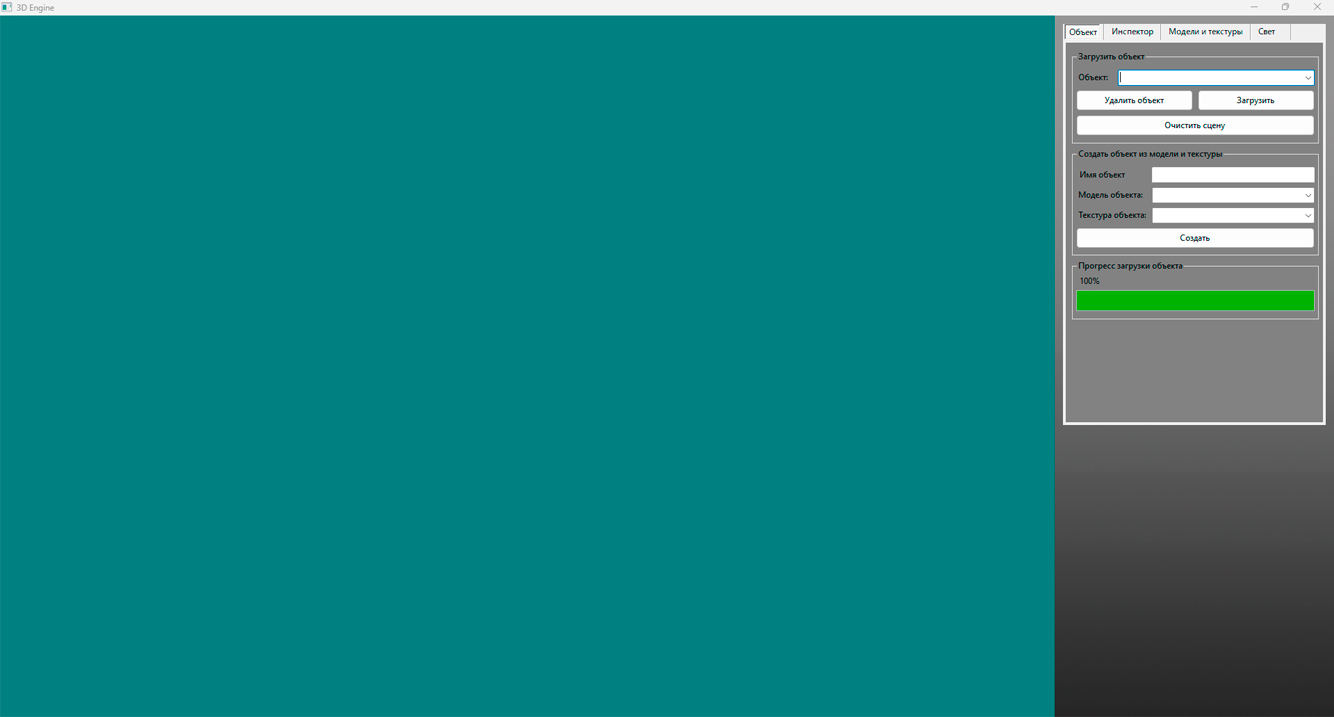
\includegraphics[width=1\linewidth]{screen1_compressed.jpg}}
	\caption{Интерфейс программы с двумя окнами}
	\label{screen1:image}
\end{figure}

Далее необходимо убедиться, что все объекты и данные ресурсов, которые указаны в примере файлов Resources.data и Objects.data в ПРИЛОЖЕНИИ В, были интерпретированы и загружены в программу.

При нажатии на контекстное меню напротив надписи "<Объект">, появляется выпадающий список, как показано на рисунке ~\ref{screen2:image}, содержащий все загруженные программой объекты, указанные в файле Objects.data.

\begin{figure}[H]
	\center{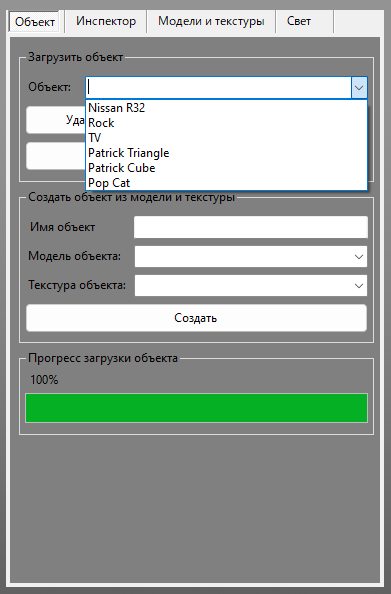
\includegraphics[width=0.6\linewidth]{screen2.png}}
	\caption{Объекты, инициализированные программой}
	\label{screen2:image}
\end{figure}

При нажатии на контекстное меню напротив надписей "<Модель объекта"> и "<Текстура объектов">, появляются выпадающие списки, содержащие ресурсы, загруженные программой при запуске, как показано на рисунках ~\ref{screen3:image} и ~\ref{screen4:image}.

\begin{figure}[H]
	\center{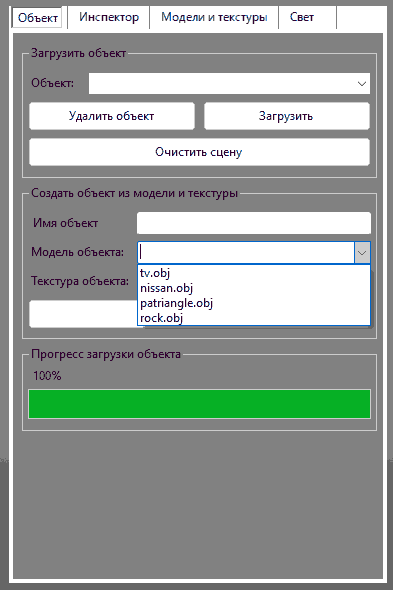
\includegraphics[width=0.6\linewidth]{screen3.png}}
	\caption{Список моделей, загруженныз в проект}
	\label{screen3:image}
\end{figure}

\begin{figure}[H]
	\center{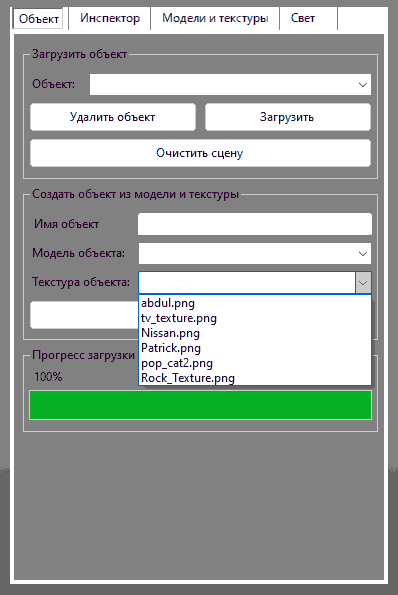
\includegraphics[width=0.6\linewidth]{screen4.png}}
	\caption{Список текстур, загруженных в проект}
	\label{screen4:image}
\end{figure}

На данных изображениях видно, что программа успешно загрузила все объекты и ресурсы, которые были указаны в файлах хранения данных.

\subsubsection{Тестовый случай: Визуализация объекта на сцене}
Действия пользователя: Пользователь пытается загрузить выбранный объект из выпадающего списка объектов на виртуальную сцену.

Ожидаемый результат: Выбранный пользователем объект корректно отображается на виртуальной сцене в главном окне программы.

Ход выполнения:

В открывшемся окне инспектора, пользователь открывает выпадающий список объектов, и выбирает строку с желаемым именем объектом. После чего, нажимает на кнопку "<Загрузить"> и запускается процесс отрисовки трёхмерного объекта. Прогресс визуализации можно наблюдать по шкале прогресса в окне инспектора чуть ниже, в разделе "<Прогресс загрузки">.

\begin{figure}[H]
	\center{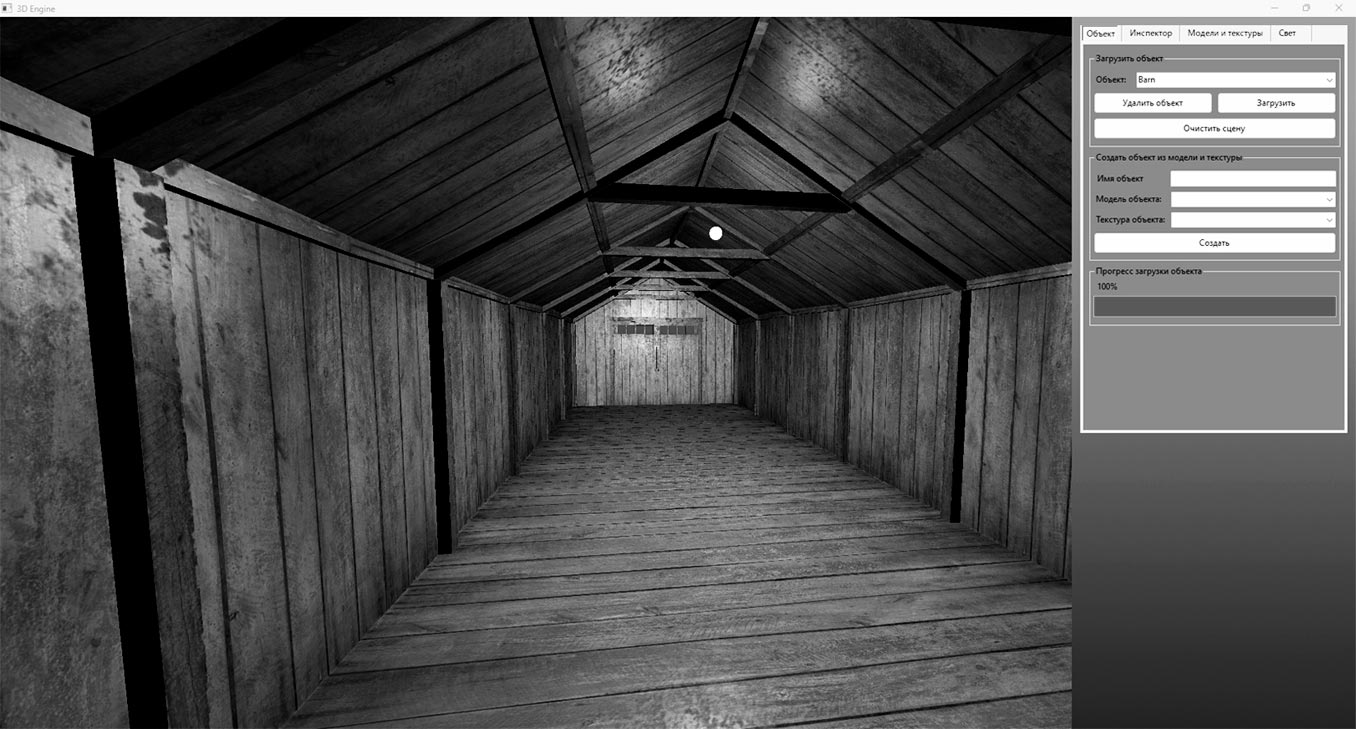
\includegraphics[width=1\linewidth]{screen15_compressed.jpg}}
	\caption{Главное окно программы с корректно отрисованным объектом на сцене}
	\label{screen15:image}
\end{figure}

После окончания визуализации объекта, пользователь увидит его в главном окне программы и сможет управлять перемещением камеры, настройкой света и выполнять трансформации над загруженным объектом.

\subsubsection{Тестовый случай: Настройка освещения}
Действия пользователя: Пользователь изменяет параметры источника света: цвет освещения - пытается ввести некорректные значения цвета в HEX формате, интенсивность общего света, интенсивность рассеянного света, интенсивность отраженного света и интенсивность отражения цвета.

Ожидаемый результат: Некорректные значения цвета в HEX формате преобразовываются в нейтрально белый цвет по умолчанию, источник света изменяет свои параметры в соответствии с веденными пользователем значениями.

Ход работы:

Для того, чтобы редактировать параметры света, необходимо, чтобы на сцене был загружен какой-либо объект, в противном случае изменение параметров света не будет иметь значения, так как не будет поверхностей, от которых свет мог бы отражаться.

В запущенной программе, пользователь переходит на вкладку инспектора "<Свет">. В открытой вкладке пользователь пытается ввести некорректные значения света в HEX-формате, как показано на рисунке ~\ref{screen17:image}. 

\begin{figure}[H]
	\center{
\includegraphics[width=0.7\linewidth]{screen17.png}}
	\caption{Пример некорректно введённого значения цвета в формате HEX}
	\label{screen17:image}
\end{figure}

После попытки применить данный некорректно введенный цвет к освещению, нажав на кнопку "<Выбрать цвет">, программа преобразует его в нейтрально белый цвет по умолчанию, как показано на рисунке ~\ref{screen18:image}.

\begin{figure}[H]
	\center{
\includegraphics[width=0.7\linewidth]{screen18.png}}
	\caption{Результат преобразования некорректного значения цвета HEX в нейтрально белый цвет}
	\label{screen18:image}
\end{figure}

Далее пользователь вводит остальные значения света, как в примере на рисунке ~\ref{screen16:image}.

\begin{figure}[H]
	\center{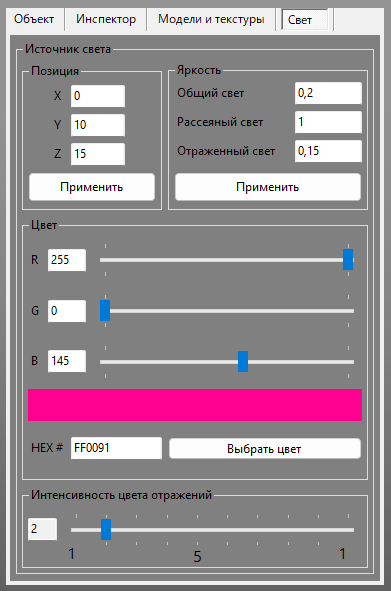
\includegraphics[width=0.6\linewidth]{screen16.png}}
	\caption{Пример введёных значений параметров света}
	\label{screen16:image}
\end{figure}

По мере введения данных значений, пользователь уже начнёт замечать изменения освещения. Ползунки, отвечающие за интенсивность одного из трёх цветов, применяют изменения к освещению сразу же, как только пользователь начал взаимодействовать с данным элементом интерфейса. Также моментально применяет свои значения и ползунок интенсивности отражения цвета.

Для применения изменения позиции и интенсивности света, необходимо нажать на кнопки "<Применить"> в соответствующих разделах поля.

Результат конечных изменений параметров света показан на рисунке ~\ref{screen19:image}.

\begin{figure}[H]
	\center{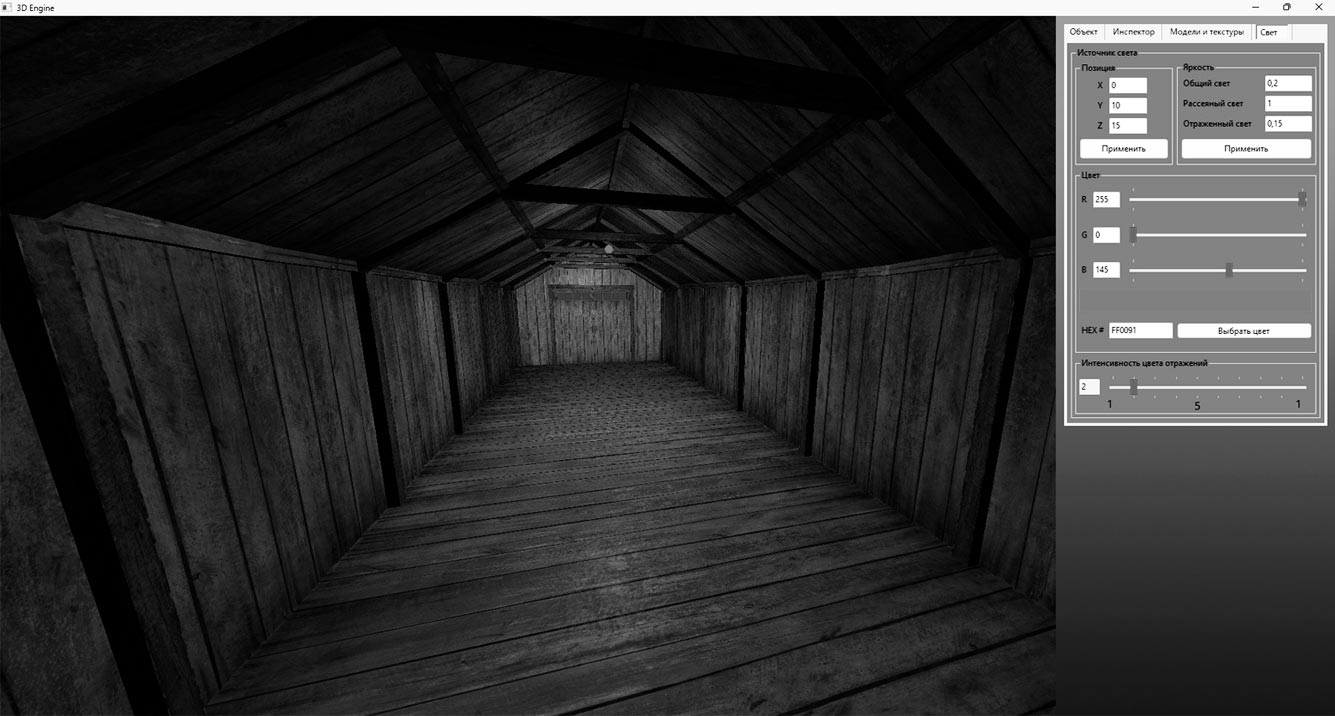
\includegraphics[width=1\linewidth]{screen19_compressed.jpg}}
	\caption{Результат изменений параметров света на виртуальной сцене}
	\label{screen19:image}
\end{figure}

\subsubsection{Тестовый случай: Трансформация объекта}
Действия пользователя: Пользователь загружает объект и пытается применить к нему трансформацию, вводя различные значения, включая отрицательные и значения, равные нулю.

Ожидаемый результат: Модель объекта, загруженного на сцену будет трансформирована, соответственно введенным пользователем значениям.

Ход выполнения:

Пользователь загружает объект на сцену, затем перейдя во вкладку "<Инспектор">, вводит значения трансформации модели объекта в соответствующие строки, как показано в примере на рисунке ~\ref{screen20:image}.

\begin{figure}[H]
	\center{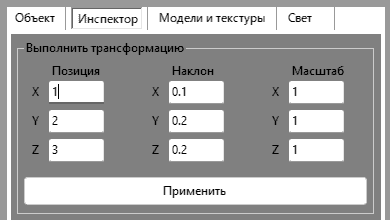
\includegraphics[width=0.6\linewidth]{screen20.png}}
	\caption{Пример введенных значений трансформации модели}
	\label{screen20:image}
\end{figure}

Чтобы применить данные трансформации, пользователь нажимает на кнопку "<Применить">. И результат становится виден на экране, как показано на рисунке ~\ref{screen21:image}.

\begin{figure}[H]
	\center{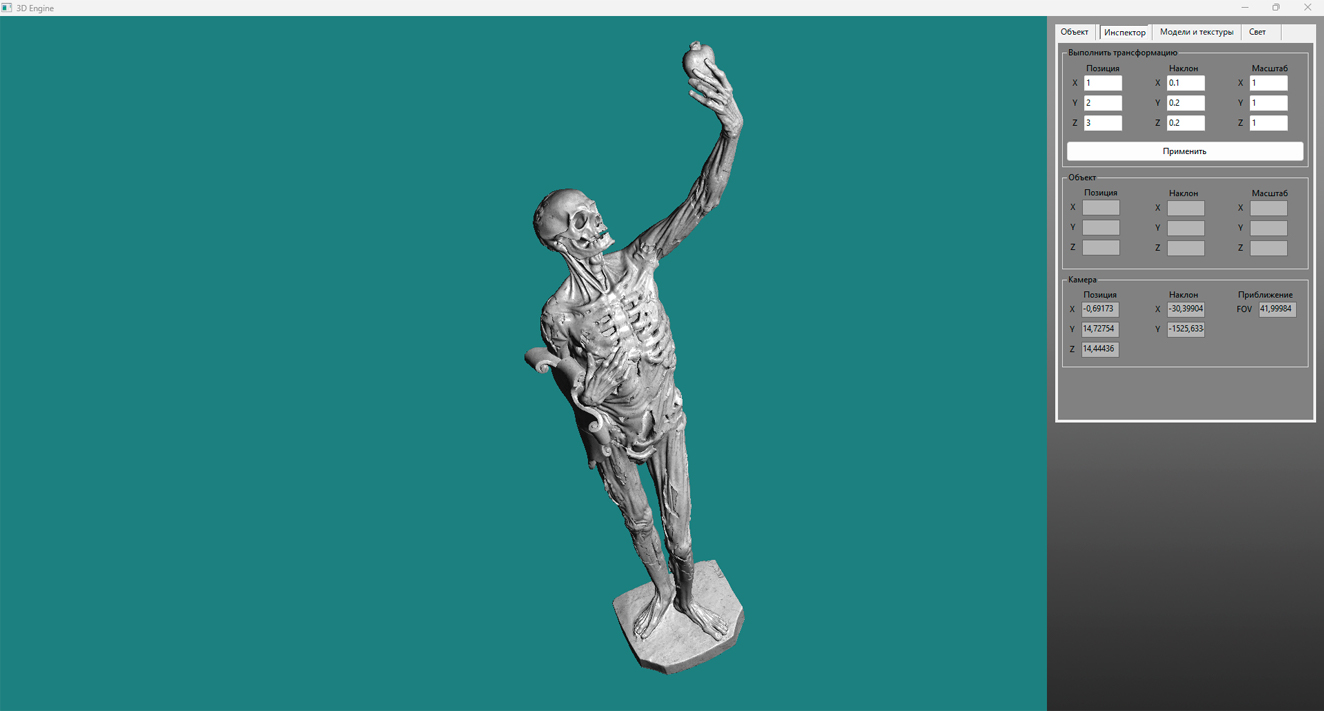
\includegraphics[width=1\linewidth]{screen21_compressed.jpg}}
	\caption{Результат трансформации трёхмерной модели объекта}
	\label{screen21:image}
\end{figure}

Как видно на снимке экрана, модель наклонилась набок, по осям в определенных значениях, указанным пользователем.

Все значения трансформаций, кроме значений масштаба модели могут быть равны нулю и отрицательными. Но в данном случае пользователь пытается задать нулевые значения для трансформации масштаба модели, как показано на рисунке ~\ref{screen22:image}

\begin{figure}[H]
	\center{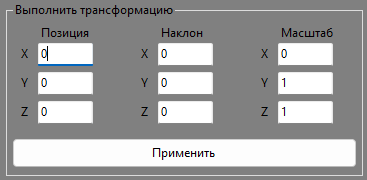
\includegraphics[width=0.6\linewidth]{screen22.png}}
	\caption{Трансформация масштаба, равная нулю в одной из координат}
	\label{screen22:image}
\end{figure}

Трансформация масштаба - это коэффициент матрицы, проще говоря число, на которое будет умножена матрица трёхмерной модели. Соответственно, при умножении матрицы на ноль, модель объекта по своей сути умножается на ноль и перестаёт существовать, так что пользователь будет наблюдать пустую виртуальную сцену.

\subsubsection{Тестовый случай: Импортирование ресурсов в проект}
Действия пользователя: Пользователь пытается загрузить собственные файлы моделей или текстур в проект со своего устройства, для дальнейшей работы с ними.

Ожидаемый результат: Файлы будут успешно загружены в проект, а пользователь сможет с ними взаимодействовать внутри программы.

Ход выполнения:

В открытой программе пользователь, переключившись на окно Инспектора, переходит во вкладку "<Модели и текстуры">, как показано на рисунке ~\ref{screen5:image}.

\begin{figure}[H]
	\center{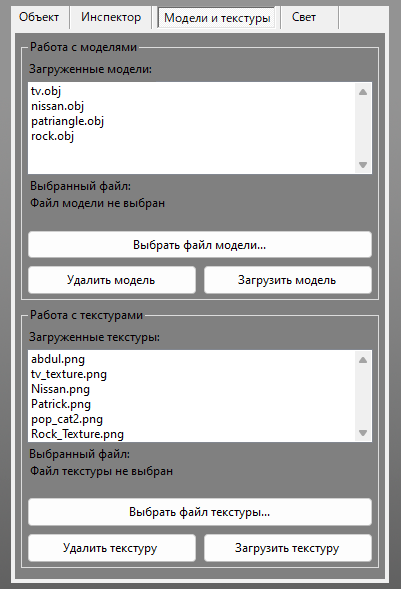
\includegraphics[width=0.6\linewidth]{screen5.png}}
	\caption{Открытая вкладка инспектора "<Модели и текстуры">}
	\label{screen5:image}
\end{figure}

На активном окне вкладки "<Модели и текстуры"> пользователь может видеть списки моделей и текстур, уже загруженные в проект. В зависимости от типа загружаемого файла в проект, пользователь нажимает на соответствующую кнопку. В данном случае пользователь желает загрузить файл трёхмерной модели объекта, и нажимает на кнопку "<Загрузить модель">. На экране появляется новое диалоговое окно с функцией выбора файла из системы устройства пользователя. Данное окно показано на рисунке ~\ref{screen6:image}.

\begin{figure}[H]
	\center{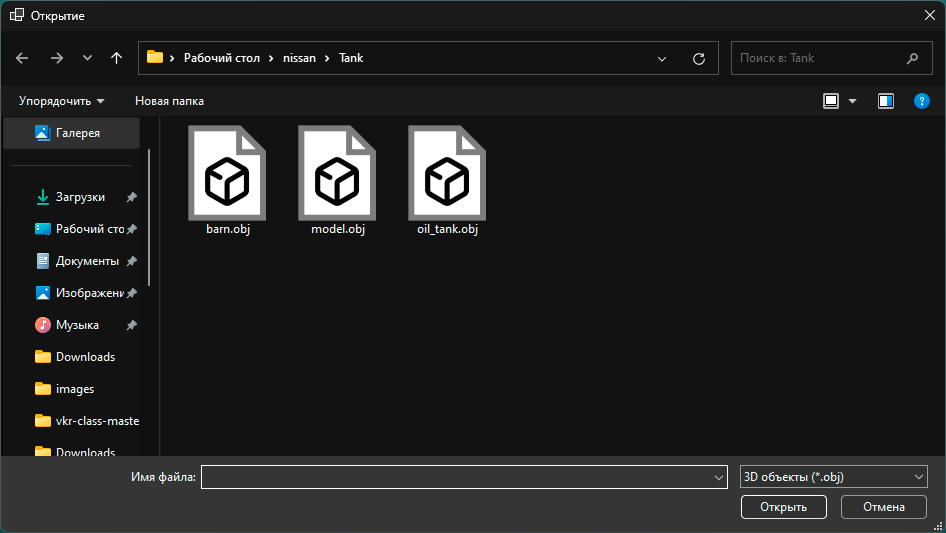
\includegraphics[width=0.75\linewidth]{screen6.jpg}}
	\caption{Диалоговое окно выбора файла}
	\label{screen6:image}
\end{figure}

В данном окне пользователь выбирает желаемый файл трёхмерной модели и нажимает на кнопку "<Открыть">. Если данный файл уже был загружен в проект, то на экране появится диалоговое окно, информирующее пользователя о перезаписи существующего файла. После окончания загрузки файла в проект, то появится диалоговое окно, информирующее пользователя об успешном импорте файла в проект (рисунок ~\ref{screen7:image}).

\begin{figure}[H]
	\center{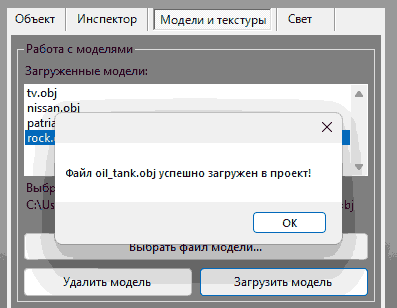
\includegraphics[width=0.75\linewidth]{screen7.png}}
	\caption{Диалоговое окно успешного импорта файла}
	\label{screen7:image}
\end{figure}

После загрузки файла, необходимо проверить корректно ли прошёл импорт. Пользователь переходит во вкладку "<Объект"> и нажимает на строку выпадающего списка того же типа, которого и был раннее загружен файл в проект. Так как пользователь загружал модель, то и нажмёт он на список, содержащий трёхмерные модели в проекте. Результат показан на рисунке ~\ref{screen8:image}.

\begin{figure}[H]
	\center{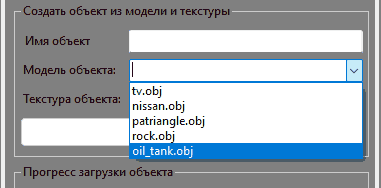
\includegraphics[width=0.8\linewidth]{screen8.png}}
	\caption{Список загруженных моделей в проект}
	\label{screen8:image}
\end{figure}

Как видно на снимке экрана, в конец выпадающего списка моделей добавилась новая позиция с наименованием файла модели oil\_tank.obj, который и загрузил пользователь немного раннее.

\subsubsection{Тестовый случай: Удаление ресурсов из проекта}
Действия пользователя: Пользователь выполняет действия для удаления соответствующего ресурса из проекта.

Ожидаемый результат: Файлы ресурсов, их ассоциации и объекты, связанные с данными ресурсами будут удалены из проекта, без возможности дальнейшего взаимодействия с ними.

Ход выполнения:

В открытой программе пользователь, переключившись на окно Инспектора, переходит во вкладку "<Модели и текстуры">.

На активном окне вкладки "<Модели и текстуры"> пользователю предоставляются списки моделей и текстур, находящиеся в проекте. В данных списках пользователь выбирает желаемый ресурс для удаления, нажав на его имя. После того, как желаемый ресурс будет выделен, пользователь нажимает на кнопку "<Удалить модель">. На экране высвечивается сообщение об успешном удалении модели из проекта. 

Но в случаях, когда данная модель являлась составляющей какого-либо существующего объекта в программе, то пользователю будет высвечено сообщение со списком объектов, которые были уничтожены, в связи с удалением их трёхмерной модели из проекта, как показано на рисунке ~\ref{screen9:image}.

\begin{figure}[H]
	\center{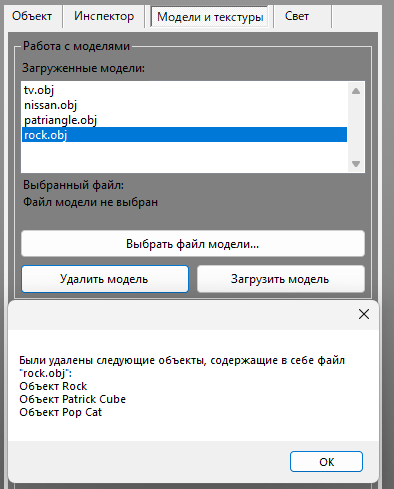
\includegraphics[width=0.8\linewidth]{screen9.png}}
	\caption{Вывод сообщения со списком удаленных объектов в проекте}
	\label{screen9:image}
\end{figure}

Перейдя во вкладку "<Объект">, и открыв выпадающий список моделей, можно увидеть на рисунке ~\ref{screen10:image}, что модель удаленного файла, также была удалена из списка прогружаемых моделей в проекте.

Далее, открыв выпадающий список объектов, можно увидеть на рисунке ~\ref{screen11:image}, что объекты, содержащие удаленную модель, также были удалены из проекта.

\begin{figure}[H]
	\center{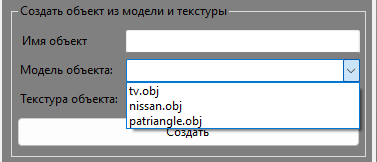
\includegraphics[width=0.8\linewidth]{screen10.png}}
	\caption{Список, демонстрирующий оставшиеся модели проекта, после удаления файла rock.obj}
	\label{screen10:image}
\end{figure}

\begin{figure}[H]
	\center{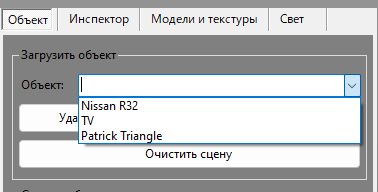
\includegraphics[width=0.8\linewidth]{screen11.png}}
	\caption{Список, демонстрирующий оставшиеся объекты в проекте, после удаления файла rock.obj}
	\label{screen11:image}
\end{figure}

\subsubsection{Тестовый случай: Создание нового объекта}
Действия пользователя: Пользователь создаёт новый объект, введя его имя и выбрав модель с текстурой.

Ожидаемый результат: В проекте создаётся новый объект, с указанным пользователем названием.

Ход работы:

В открывшемся окне инспектора, пользователь вводит желаемое имя для объекта напротив надписи "<Имя объекта">, а также выбирает модель и текстуру для данного объекта из выпадающих списков чуть ниже. Корректное и полное заполнение полей для создания объекта показано на рисунке ~\ref{screen12:image}.

\begin{figure}[H]
	\center{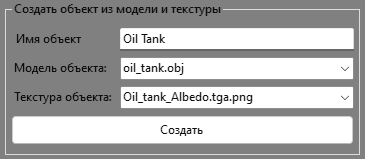
\includegraphics[width=0.8\linewidth]{screen12.png}}
	\caption{Пример корректного заполнения полей для создания нового объекта}
	\label{screen12:image}
\end{figure}

Нажав на кнопку "<Создать">, система уведомит об успешном создании объекта с указанным именем.

Теперь пользователь может загрузить на сцену только что созданный объект. На той же вкладке, открыв выпадающий список объектов, в его конце появится имя нового объекта (рисунок ~\ref{screen13:image}).

\begin{figure}[H]
	\center{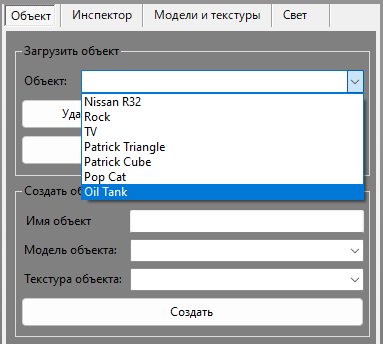
\includegraphics[width=0.8\linewidth]{screen13.png}}
	\caption{Обновленный список объектов, в который был добавлен объект Oil Tank}
	\label{screen13:image}
\end{figure}

После того, как в проект был добавлен объект с указанным именем и связанными с ним моделью и текстурой, можно проверить корректность его отображения на виртуальной сцене. Выбрав имя объекта в выпадающем списке, и нажав на кнопку "<Загрузить">, в главном окне программы будет отрисован текущий объект. Результат визуализации нового объекта показан на рисунке ~\ref{screen14:image}.

\begin{figure}[H]
	\center{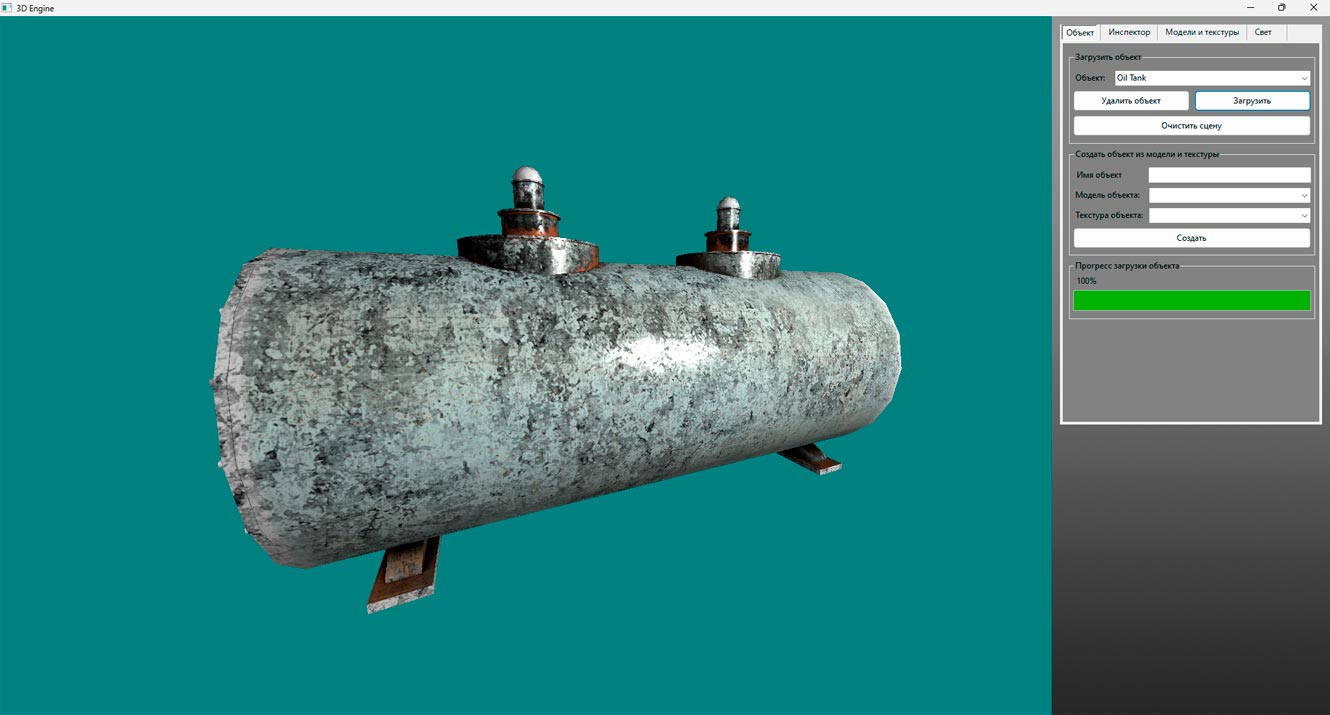
\includegraphics[width=1\linewidth]{screen14_compressed.jpg}}
	\caption{Результат визуализации объекта на сцене, созданного пользователем}
	\label{screen14:image}
\end{figure}

На данном снимке экрана можно увидеть, что модель и текстура объекта на виртуальной сцене отображена корректно.